%!TEX root = paper.tex

\section{The Spack Package Manager}
\label{sec:implementation}
Based on our experiences at LLNL, we have developed
{\it Spack}, the Supercomputing PACKage manager.
Spack is written in Python.  We chose Python for its flexibility
and its wide use in the HPC community.
%
Like prior systems, Spack supports an arbitrary number of software
installations, and like Nix it can identify them with hashes.  Unlike any
prior system, Spack provides a language to specify and manage the
combinatorial space of HPC software configurations.

\noindent
Spack has the following unique capabilities:
\begin{enumerate}
\item Packages are {\bf parameterized}, allowing new builds to be composed
      on the fly for different versions, architecture, compiler, options, 
      and dependencies.
\item To manage this large parameter space, spack provides a novel, 
      recursive {\bf spec syntax} for dependency graphs.
\item Specs support versioned, ABI-incompatible interfaces like MPI through
      {\bf versioned virtual dependencies}.
\item Spack builds with {\bf compiler wrappers} that enforce build
      consistency and simplify package writing.
\end{enumerate}

%!TEX root = paper.tex

\subsection{Packages}

%\subsubsection{Package Files}
\begin{figure}
	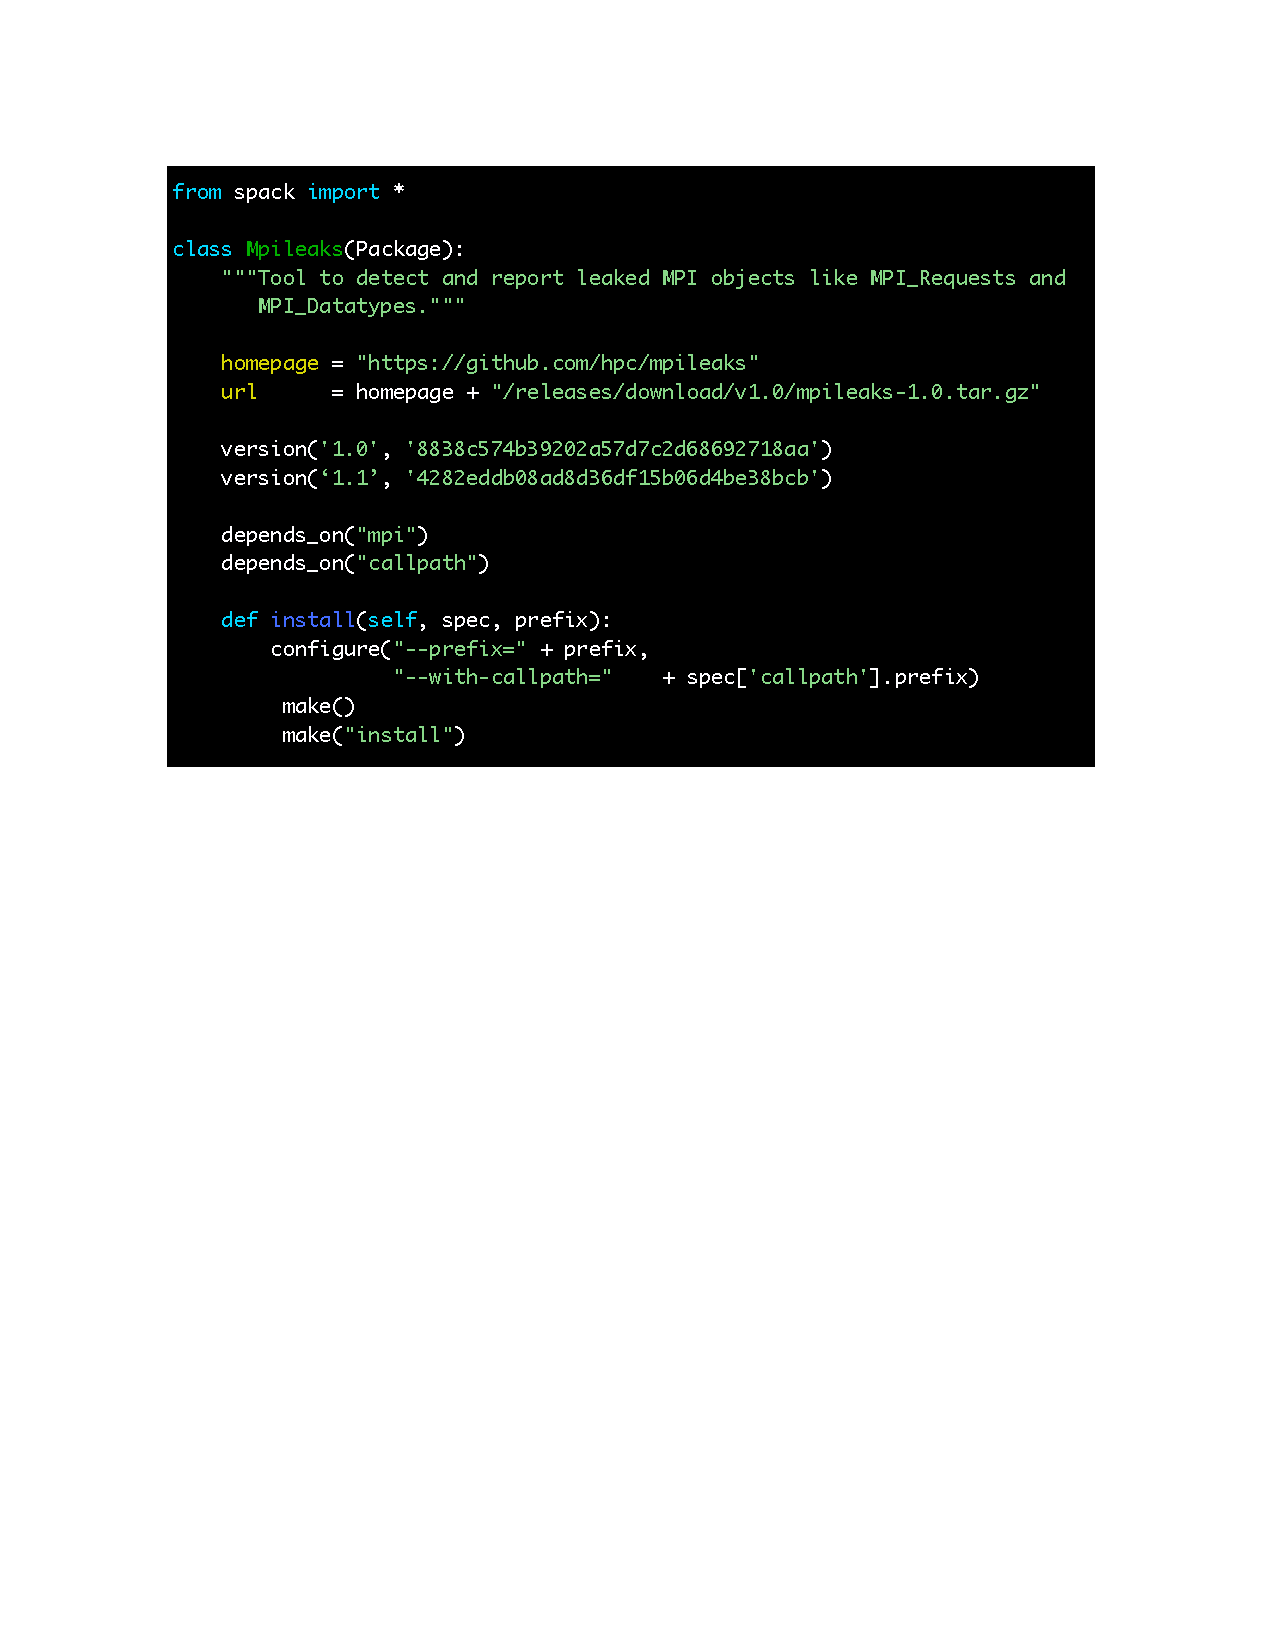
\includegraphics[width=\columnwidth]{code/mpileaks.pdf}
	\caption{
		Spack package for the {\tt mpileaks} tool.
		\label{fig:mpileaks}
	}
\end{figure}

In Spack, packages are build scripts that describe how to build software
artifacts.  Each package is a class written in pure Python to describe
{\it specific} build instructions, and it must extend the {\tt Package}
base class, which implements the more general parts of the build process.
Spack implements a simple, embedded domain-specific language (DSL) to make
packaging easier; it adds special directives such as {\tt depends\_on} and
{\tt version} that add metadata to the class.

Figure~\ref{fig:mpileaks} shows the package for \mpileaks, an LLNL-developed
tool for finding leaks in MPI programs.
Inside the {\tt MpiLeaks} class, the package provides a text description
and a homepage, as well as 
a download URL.  Next, two {\tt version} directives identify known versions
of the package, and MD5 checksums ensure they can be downloaded safely.
Below this, two {\tt depends\_on}
directives indicate prerequisites that must be installed before \mpileaks.
Last, each package defines an {\tt install()} method, which contains the
commands used to build the package.  Spack's DSL allows shell
commands to be invoked as Python functions. Here, the {\tt install()} 
method invokes the familiar {\tt configure}, {\tt make}, and
{\tt make install} build commands, as a shell script would.






%!TEX root = spack-sc15.tex

\begin{figure}
	\begin{subfigure}{\linewidth}
		\centering
		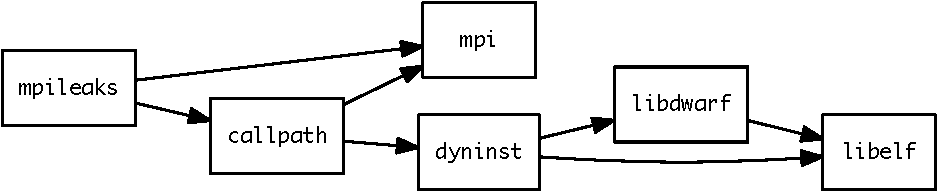
\includegraphics[width=.9\columnwidth]{specs/mpileaks.pdf}
		\caption{
			Spec for {\tt mpileaks}
			\label{fig:specs-mpileaks}
		}
	\end{subfigure}
%
	\begin{subfigure}{\linewidth}
		\centering
		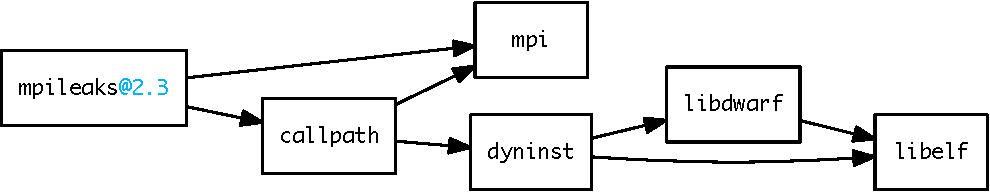
\includegraphics[width=.9\columnwidth]{specs/mpileaks-version}
		\caption{
			{\tt mpileaks@2.3}
			\label{fig:specs-mpileaks-version}
		}
	\end{subfigure}
%
	\begin{subfigure}{\linewidth}
		\centering
		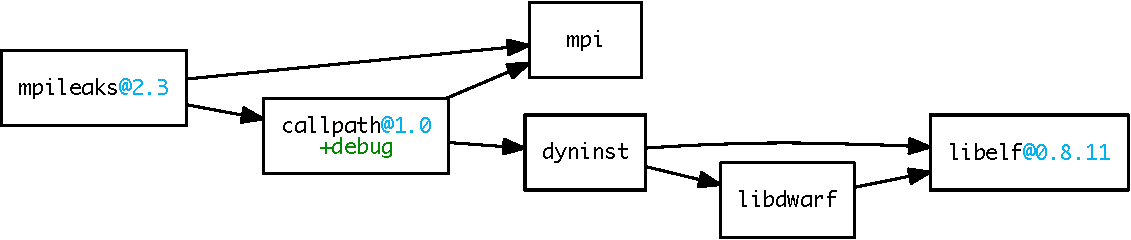
\includegraphics[width=.9\columnwidth]{specs/mpileaks-abstract.pdf}
		\caption{
			{\tt mpileaks@2.3 \^{}callpath@1.0+debug \^{}libelf@0.8.11}
			\label{fig:specs-mpileaks-abstract}
		}
	\end{subfigure}
%
	\caption{
		Constraints applied to {\tt mpileaks} specs.
	}
	\label{fig:specs}
\end{figure}



\subsection{Spack Specs}\label{sec:specs}

Using the simple script in Figure~\ref{fig:mpileaks}, Spack can build many different
versions and configurations of the {\tt mpileaks} package.  In traditional port systems,
package code is structured to build a single version of a package, but in Spack, each
package file is a {\it template} that can be configured and built in many
different ways, according to a set of {\it parameters}.
Spack calls a single build configuration a {\it spec}.
Spack communicates dependencies and parameters to package authors using
the {\tt spec} argument of the {\tt install} method.

\subsubsection{Structure}
To understand specs, consider the {\tt mpileaks} package structure.
Metadata in the {\tt Mpileaks} class (e.g., {\tt version} or
{\tt depends\_on}) describe its relationships with other packages.
The tool has two direct dependencies:
the {\tt callpath} library and {\tt mpi}.  Spack recursively inspects the class definitions
for each dependency and constructs a graph of their relationships.  The result
is a directed, acyclic graph (DAG).\footnote{Spack currently disallows
circular dependencies.}
%
To guarantee a consistent build and to avoid
Application Binary Interface (ABI) incompatibility, we construct
the DAG with only {\it one} version of each package.  Thus, while
Spack can install arbitrarily many configurations of any package,
no two configurations of the same package will ever appear in the same build DAG.

DAGs for {\tt mpileaks} are shown in Figure~\ref{fig:specs}.
Each node represents a package, and each package has five configuration parameters that control
how it will be built: 1) the package version, 2) the compiler with which to
build, 3) the compiler version, 4) named compile-time build options, or
{\it variants}, and 5) the target architecture.


\subsubsection{Configuration Complexity}
A spec DAG has many degrees of freedom, and users cannot reasonably be
expected to understand or to specify all of them.  In our experience at LLNL,
the typical user only cares about a small number of build constraints (if any),
and does not know enough to
specify the rest. For example, a user may know that a certain version of a library like
{\tt boost}~\cite{boost} is required, but only cares that other build parameters are set so that
the build will succeed.
%
Configuration complexity makes the HPC software ecosystem difficult to manage:
too many parameters exist to specify them all. However, the known and
important ones often provide detailed build constraints. Thus, we have two
competing concerns.  We need the ability to specify details
without having to remember all of them.

\subsubsection{Spec Syntax}\label{sec:syntax}
\begin{figure}
{\fontfamily{cmr}\selectfont
\begin{grammar}\small
  <spec>         ::= <id> [ <constraints> ]

  <constraints>   ::= \{ `@' <version-list> | `+' <variant> \newline
                   | `-' <variant> ~~~| `~' <variant> \newline
                   | `\%' <compiler> ~| `=' <architecture> \} \newline
                  [ <dep-list> ]

  <dep-list>  ::= \{ `\textsf \textasciicircum' <spec> \}

  <version-list> ::= <version> [ \{ `,' <version> \} ]

  <version>      ::= <id> | <id> `:' | `:' <id> | <id> `:' <id>

  <compiler>     ::= <id> [ <version-list> ]

  <variant>      ::= <id>

  <architecture> ::= <id>

  <id>           ::= "[A-Za-z0-9_][A-Za-z0-9_.-]*"
\end{grammar}
} % End fontfamily{cmr}
\caption{
	EBNF grammar for spec expressions.
	\label{fig:grammar}
}
\end{figure}


\begin{table*}\centering
\begin{tabular}{|r|p{2.4in}|p{4in}|}
\hline
& {\bf Spec} & {\bf Meaning} \\
\hline
\hline
1&\small\verb|mpileaks|                         & \small {\tt mpileaks} package, no constraints. \\\hline
2&\small\verb|mpileaks@1.1.2|                   & \small {\tt mpileaks} package, version 1.1.2. \\\hline
3&\small\verb|mpileaks@1.1.2 %gcc|              & \small {\tt mpileaks} package, version 1.1.2, built with {\tt gcc} at the default version. \\\hline
4&\small\verb|mpileaks@1.1.2 %intel@14.1 +debug| & \small {\tt mpileaks} package, version 1.1.2, built with Intel compiler version 14.1, \newline with the ``debug'' build option. \\\hline
5&\small\verb|mpileaks@1.1.2 =bgq|              & \small {\tt mpileaks} package, version 1.1.2, built for the Blue Gene/Q platform (BG/Q). \\\hline
6&\small\verb|mpileaks@1.1.2 ^mvapich2@1.9|     & \small {\tt mpileaks} package version 1.1.2, using {\tt mvapich2}  version 1.9 for MPI. \\\hline
7&\small\verb|mpileaks @1.2:1.4 %gcc@4.7.5 -debug =bgq| \newline
      \verb|  ^callpath @1.1 %gcc@4.7.2| \newline
      \verb|  ^openmpi @1.4.7|                & \small%
      {\tt mpileaks} at any version between 1.2 and 1.4 (inclusive), built with gcc 4.7.5,
      without the debug option, for BG/Q, linked with {\tt callpath} version 1.1
      and building {\tt callpath} with {\tt gcc} version 4.7.2, linked with {\tt openmpi} version 1.4.7.    \\
\hline
\end{tabular}
\caption{
	Spack build spec syntax examples and their meaning.
	\label{tab:specs}
}
\end{table*}

We have developed a syntax for specs that allows users to specify
only constraints that matter to them. Our syntax can represent
DAGs concisely enough for command line use.
The spec syntax is recursively defined to allow users to specify
parameters on dependencies as well as on the root of the DAG.
Figure~\ref{fig:grammar} shows the EBNF grammar through which Spack
flexibly supports constraints.

We begin with a simple example.
Consider the case where a user wants to install the {\tt mpileaks} package, but knows
nothing about its structure.  To install the package, the user invokes {\tt spack install}:
%
\begin{minted}[fontsize=\scriptsize]{bash}
    $ spack install mpileaks
\end{minted}
%
Here, {\tt mpileaks} is the simplest possible spec---a single identifier.
Spack converts it into the DAG shown in Figure~\ref{fig:specs-mpileaks}.
Note that even though the spec contains no dependency information, it is still
converted to a full DAG, based on directives supplied in package files. Since
the spec does not constrain the nodes, Spack has leeway when building the
package, and we say that it is {\it unconstrained}.
%
However, a user who wants a specific {\tt mpileaks} version can
request it with a version constraint after the package name:
%
\begin{minted}[fontsize=\scriptsize]{bash}
    $ spack install mpileaks@2.3
\end{minted}
%
Figure~\ref{fig:specs-mpileaks-version} shows that the specific version
constraint is placed on the {\tt mpileaks} node in the DAG, which otherwise
remains unconstrained.
A user who only requires a particular minimum version could use
{\it version range} syntax
and write {\tt @2.3:}.  Likewise, {\tt @2.3:2.5.6} would specify a
version between 2.3 and 2.5.6. In these cases, the user can save time if
Spack already has a version installed that satisfies the spec -- Spack will use
the previously-built installation instead of building a new one.

Figure~\ref{fig:specs-mpileaks-abstract} shows the recursive nature of the spec syntax:
%
\begin{minted}[fontsize=\scriptsize]{bash}
    $ spack install mpileaks@2.3 ^callpath@1.0+debug ^libelf@0.8.11
\end{minted}
%
The caret (\verb|^|) denotes constraints for a particular dependency. The DAG
now has version constraints on {\tt callpath} {\it and} {\tt libelf},
and the user has requested the {\tt debug} variant of the {\tt callpath} library.

Recall that Spack guarantees that only a single version of any package occurs
in a spec.  Within a spec, each dependency can be uniquely
identified by its package name alone.  Therefore, the user does not need to consider
DAG connectivity to add constraints but instead must only know that
{\tt mpileaks} depends on {\tt callpath}.
Thus, dependency constraints can appear in an arbitrary order.

Table~\ref{tab:specs} shows further examples of specs, ranging from
simple to complex. These examples show how Spack's constraint
notation covers the rest of the HPC package parameter space.

{\bf Versions.}
Version constraints are denoted with {\tt @}. Versions
can be precise ({\tt @2.5.1}) or denote a range ({\tt @2.5:4.4}),
which may be open-ended ({\tt @2.5:}).
%
The package in Figure~\ref{fig:mpileaks} lists two ``safe'' versions with
checksums, but
in our experience users frequently want bleeding-edge versions, and package managers
often lag behind the latest releases.
Spack can extrapolate URLs from versions,
using the package's {\tt url} attribute as a model.\footnote{This works
for packages with consistently named URLs.}  If the user requests a specific
version on the command line that is unknown to Spack,
Spack will attempt to fetch and to install it.  Spack uses the same
model to scrape webpages and to find new versions as they become available.

\begin{figure}
\begin{minted}[linenos,
               numbersep=5pt,
			   fontsize=\scriptsize,
               frame=lines,
               framesep=2mm]{python}
    def install(self, spec, prefix):  # default build uses cmake
        with working_dir('spack-build', create=True):
            cmake('..', *std_cmake_args)
            make()
            make("install")

    @when('@:8.1')                    # <= 8.1 uses autotools
    def install(self, spec, prefix):
        configure("--prefix=" + prefix)
        make()
        make("install")
\end{minted}
\caption{
    Specialized {\tt install} method in Dyninst.
	\label{fig:specialization}
}
\end{figure}

{\bf Compilers.}
With a compiler constraint (shown on line 3) the user
simply adds {\tt \%} followed by its name, with an optional compiler version
specifier.  Spack compiler names like {\tt gcc} refer to the full compiler {\it toolchain},
i.e., the C, C++, and Fortran 77 and 90 compilers.  Spack can auto-detect
compiler toolchains in the user's {\tt PATH}, or they can be registered manually
through a configuration file.

{\bf Variants.}
To handle options like compiler flags or optional components, specs can
have named flags, or {\it variants}.  Variants are associated with the package,
so the {\tt mpileaks} package implementer must explicitly handle cases
where debug is enabled ({\tt +debug}) or disabled ({\tt -debug}
or {\tt \textasciitilde \ignorespaces debug}).  Names simplify versioning
and prevent the configuration space from becoming too large.
For example, including detailed compiler flags in spec syntax
would violate our goal of conciseness, but known sets of flags can simply be named.

{\bf Cross-compilation.}
To support cross-compilation, specs can include the system architecture
(line 5). Platforms begin with {\tt =} and take names like {\tt linux-ppc64}
or {\tt bgq}.  They are specified per-package. This mechanism allows front-end
tools to depend on their back-end measurement
libraries with a {\it different} architecture on cross-compiled machines.

\subsubsection{Constraints in Packages}\label{sec:constraints}

So far, we have shown examples of specs used to request constraints from the
command line, when {\tt spack install} is invoked.  However, the user is not
the only source of constraints.  Applications may require specific versions
of dependencies. Often, these constraints should be specified in a package
file.  For
example, the ROSE compiler~\cite{rose} only builds with a certain version of the {\tt boost} library.
The {\tt depends\_on()} directives in Figure~\ref{fig:mpileaks} contain
simple package names.  However, a package name is also a spec, and
the same constraint syntax usable from the command line can be applied inside directives.
So, we can simply write:
%
\begin{minted}[fontsize=\scriptsize]{python}
    depends_on('boost@1.54.0')
\end{minted}
%
This constraint will be incorporated into the initial DAG node generated from
the {\tt ROSE} package.  Dependencies can also be {\it conditional}.  For example,
the {\tt ROSE} package builds with different versions of boost, depending on the
compiler version. So, directives also accept spec syntax as a
predicate in an optional {\tt when} parameter:
%
\begin{minted}[fontsize=\scriptsize]{python}
    depends_on('boost@1.47.0', when='%gcc@:4')
    depends_on('boost@1.54.0', when='%gcc@5:')
\end{minted}
%
\vfill\eject
\noindent
The same notation is used to build optionally with libraries like MPI:
%
\begin{minted}[fontsize=\scriptsize]{python}
    depends_on('mpi', when='+mpi')
\end{minted}
%
and to ensure that specific patches are applied to Python source code
when it is built on Blue Gene/Q, with different compilers:
%
\begin{minted}[fontsize=\scriptsize]{python}
    patch('python-bgq-xlc.patch',   when='=bgq%xl')
    patch('python-bgq-clang.patch', when='=bgq%clang')
\end{minted}
%
Constraints in the {\tt when} clause are matched against the package spec.
Outside of directives, constraints can also be tested directly on the {\tt spec}
object in the {\tt install} method:
%
\begin{minted}[fontsize=\scriptsize]{python}
  def install(self, spec, prefix):
      if spec.satisfies('%gcc'):
          # Handle gcc
      elif spec.satisfies('%xl'):
          # Handle XL compilers
\end{minted}
%

\subsubsection{Build Specialization}

In our experience maintaining packages at LLNL, we often must change
entire package build scripts due to large changes in the way certain packages build.
These changes are cumbersome, particularly since we often must maintain both
the old and new version of a build script, as some users rely on the old version.


%class Dyninst(Package):
%    """"Dyninst binary instrumentation and analysis tool."""
%    url="http://www.paradyn.org/release8.1/DyninstAPI-8.1.1.tgz"
%    version('8.1.1', 'd1a04e995b7aa70960cd1d1fac8bd6ac')
%    depends_on("libelf")
%    depends_on("libdwarf")
%    depends_on("boost@1.42:")
%

Spack provides functionality that allows Python functions to have
multiple definitions, each specialized for particular configurations of the package.
This capability allows us to have two separate implementations of {\tt install} or {\it any} method
in a package class, as Figure~\ref{fig:specialization} shows for the Dyninst
package.  The {\tt @when} directive is a Python decorator: a higher order function that
takes a function definition as a parameter and returns a new function to replace it.
We replace the function with a callable multi-function dispatch object, and we
integrate the predicate check into the function dispatch mechanism.  The
{\tt @when} condition is true when Dyninst is at version 8.1 or lower, in which
case the package will use the {\tt configure}-based build.  By default if no predicate matches,
{\tt install} will use the default CMake-based implementation. The simple {\tt @when}
annotation allows us to maintain our old build code alongside the new version without
accumulating complex logic in a single {\tt install} function.

%!TEX root = paper.tex


\subsection{Versioned Virtual Dependencies}
	\todo{.5 page}

%!TEX root = spack-sc15.tex

\subsection{Concretization}
\label{sec:concretization}

We have discussed Spack's internal software DAG model, and we have shown
how the spec syntax can be used to specify a partially constrained
software DAG.  This DAG is {\it abstract}, as it could potentially
describe more than one software configuration. Before Spack builds a spec, it
must ensure the following conditions:
\begin{enumerate}
\item No package in the spec DAG is missing dependencies;
\item No package in the spec DAG is virtual;
\item All parameters are set for all packages in the DAG.
\end{enumerate}
If a spec meets these criteria then it is {\it concrete}.
{\it Concretization} is the central component of Spack's build
process that allows it to reduce an unconstrained abstract
description to a concrete build.

Figure~\ref{fig:concretization} shows Spack's concretization algorithm.
The process starts when a user invokes {\tt spack install} and requests that a
spec be built.  Spack converts the spec to an abstract DAG.
It then builds a {\it separate} spec DAG for any constraints encoded
by directives in package files.
%
Spack intersects the constraints of the two DAGs package by package, and it
checks each parameter for inconsistencies.  Inconsistencies can arise if, 
for example,
the user inadvertently requests two versions of the same package, or if a
package file depends on a different version than the user requested.
Likewise, if the package and the user specified different compilers, variants,
or platforms for particular packages, Spack will stop and notify
the user of the conflict. If the user or package specifies version ranges,
they are intersected, and if the ranges do not overlap, Spack raises an error.
When the intersection succeeds, Spack has a single DAG with the merged
constraints of the user and the package files.

The next part of the process is iterative.
If any node is a virtual dependency, Spack replaces it with a
suitable interface provider by building a reverse
index from virtual packages to providers using the {\tt provides when}
directives (Section~\ref{sec:virtual}). If multiple providers
satisfy the virtual spec's constraints,
Spack consults site and user policies to select the ``best'' possible
provider.  The selected provider may {\it itself} have virtual dependencies,
so this process is repeated until the DAG has no more virtual packages.

With the now non-virtual DAG, Spack again consults site and user preferences for
variants, compilers, and versions to resolve any remaining abstract nodes.
Adding a variant like {\tt +mpi} may cause a package to depend on more
libraries (as in Section~\ref{sec:constraints}). The concretization algorithm
evaluates conditions from {\tt when} clauses on the DAG; if they result in
new libraries or other changes, the cycle begins again.
Spack currently avoids an exhaustive search by using a greedy algorithm.
It will not backtrack to try other options if its first policy choice leads
to an inconsistency.  Rather, it will raise an error and the user must resolve
the issue by being more explicit.  The user might toggle a variant or force 
the build to use a {\it particular} MPI implementation
by supplying \verb|^openmpi| or \verb|^mpich|.  We leave automatic constraint
space exploration for future work.

\begin{figure}
	\centering
	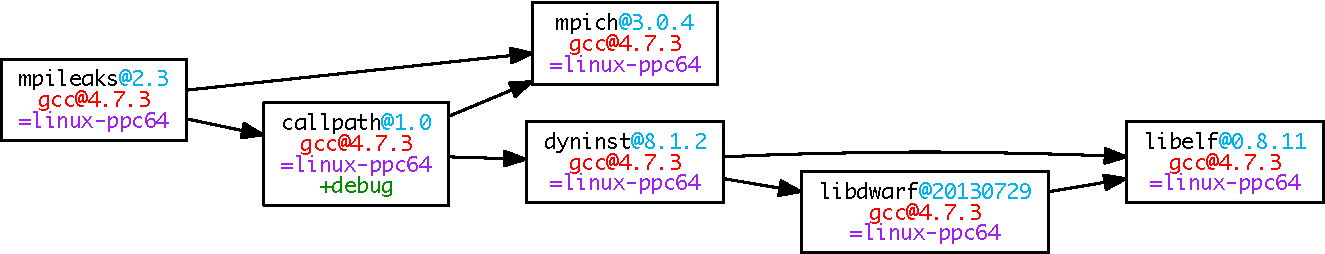
\includegraphics[width=\columnwidth]{specs/mpileaks-concrete.pdf}
	\caption{
		Concretized spec from Figure~\ref{fig:specs-mpileaks}.
		\label{fig:specs-mpileaks-concrete}
	}
\end{figure}
On completion, the concretization outputs a fully concrete spec DAG.
Figure~\ref{fig:specs-mpileaks-concrete} shows a concrete DAG with architectures,
compilers, versions, variants, and all dependencies resolved.
This fulfills Spack's guarantees.
%
At install time, Spack constructs a package object for each node in the spec DAG
and traverses the DAG in a bottom-up fashion.  At each node, it invokes the package's
{\tt install} method.  For the {\tt spec} parameter to {\tt install}, it passes
a sub-DAG rooted at current node (also a concrete spec).  Package authors must
query the spec in {\tt install} to handle different configurations.

\subsubsection{Concretization Runtime}
\label{sec:concretization-overhead}

\begin{figure}
	\centering
	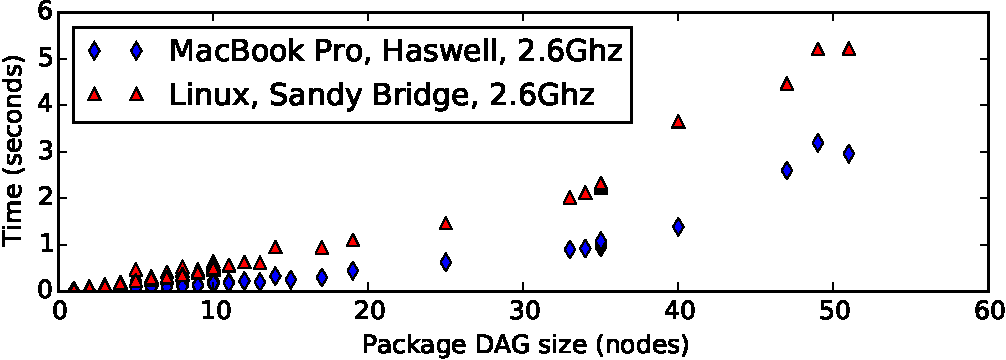
\includegraphics[width=.95\columnwidth]{figs/concretization-overhead/concretization-times.pdf}
	\caption{
		Concretization running time for 245 packages.
		\label{fig:concretization-time}
	}
\end{figure}

Figure~\ref{fig:concretization-time} shows the running time of concretization vs.
package DAG size in nodes.  We generated this plot by running {\tt concretize}
on all of Spack's 245 packages. We tested on three LLNL cluster front-end nodes:
a 2.3GHz Intel Haswell node and a 2.6 GHz Intel Sandy Bridge node on our Linux
clusters, and the 3.6 GHz IBM Power7 front-end node of a Blue Gene/Q system.
Each point is the average of 10 trials.  For all but the 10
largest packages, concretization takes less than 2 seconds on all machines.
For larger DAGs, we begin to see a quadratic trend, but even for 50 nodes or more,
concretization takes less than 4 seconds on the Haswell machine and 9 seconds on the
Power7.
%
We expect this performance from our greedy, fixed-point method, and
it is sufficient for the packages we have built so far.
Its running time is insignificant compared to the build time of
most packages, and it only executes
once per build.
More generally, concretization is an instance of the constraint
satisfaction problem, which is NP-complete. While concretization could become
more costly, we do not expect to see packages with
thousands of dependencies in the near future. We do not expect
it to become a bottleneck, even if we use a full constraint solver.

\subsubsection{Shared sub-DAGs}
\label{sec:directory-layout}

We mentioned in Section~\ref{sec:packages} that each unique configuration is
guaranteed a unique install prefix. Spack uses the concrete {\it spec}
to generate a unique path, shown in Table~\ref{tab:naming-conventions}.
To prevent the directory name from growing too long, Spack uses a SHA hash of
dependencies' specs as the last directory component.  However, Spack
does {\it not} rebuild every library for each new configuration.
If two configurations share a sub-DAG, then Spack reuses the sub-DAG's 
configuration.  Figure~\ref{fig:reuse} shows how the {\tt dyninst} sub-DAG 
is used for both the {\tt mpich} and {\tt openmpi} builds of {\tt mpileaks}.


\subsubsection{Reproducibility}


For reproducibility, and to preserve provenance, Spack stores a number of
files in the installation directory that document how the installed package was
built.  These include the {\tt package.py} file used to build, a build log
that contains output and error messages, and a file that contains the complete
concrete spec for the package {\it and} its dependencies. The spec file can be
used later to reproduce the build, even if concretization preferences have 
changed.

\subsubsection{Site policies and build complexity}

Our experience with manual installs helped us understand that much of the complexity
of building HPC software comes from the size of the build parameter space.
As previously mentioned, typical users only care about a few parameters.
The rest add unneeded complexity.  When building manually, LLNL staff
tend to make arbitrary choices about the secondary build parameters,
or they add logic to build scripts to make these choices.
Manually built software is generally not installed in a consistent manner.

Concretization provides two benefits.  First, it allows users and staff to
request builds with a minimal spec expression, while still providing a
mechanism for the site and the user to make consistent, repeatable choices 
for other build parameters.  For example, the site or the user can set 
default versions to use for any library that is not specified explicitly.
%
Second, concretization reduces the burden of packaging software, because
package authors do not have to make these decisions. Packages do not need 
to contain complicated checks, or to be overly specific about versions.  
Other multi-configuration systems like Nix, EasyBuild, and HashDist require 
the package author to write a mostly concrete build spec in advance.
This requirement puts undue burden on the package author, and it makes the task
of changing site policies within a software stack difficult.  Spack
separates these concerns.

\begin{figure}\centering
   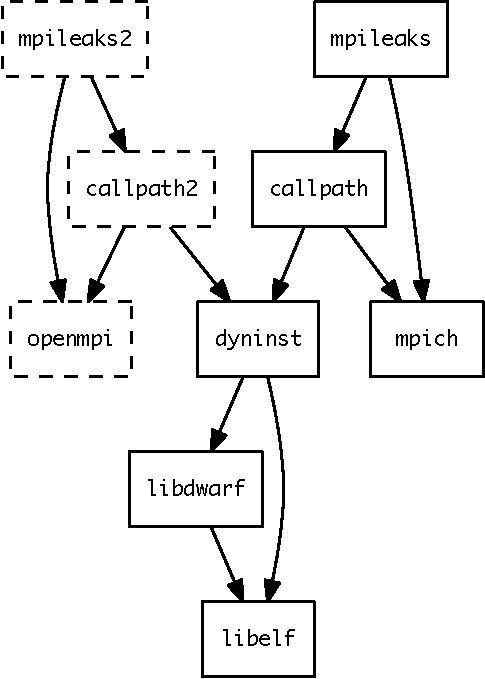
\includegraphics[width=.9\linewidth]{specs/rpaths.pdf}
   \caption{
       {\tt mpileaks} built with {\tt mpich}, then {\tt openmpi}.
       \label{fig:reuse}
   }
\end{figure}

%!TEX root = paper.tex


\subsection{Installation Environment}

%{\bf Reproducibility.}
%\paragraph{Reproducibility}
Spack is intended to build a consistent HPC stack for our multi-user
environment, and reproducible builds are one of our design goals.
Experience at LLNL has shown that it is vexingly difficult to reproduce
a build manually.
%
Many packages used at LLNL have a profusion of build options, and specifying them 
correctly often requires tedious experimentation.  This is due to lack of
build standards and to the diversity of HPC environments.  
For example, in some packages that depend on the {\tt Silo} library,
the \verb|--with-silo| parameter takes a path to {\tt Silo}'s installation prefix.
In others, it takes the {\tt include} and {\tt lib} subdirectories,
separated by a comma.
The {\tt install} method in Spack's package files allows us to record
precise build incantations for later reuse.

%{\bf Environment isolation.}
\paragraph{Environment isolation}
In addition to command-line issues, we
frequently encounter errors due to inconsistencies between the environment of
the package installer and the package user.
%
For example, there are two versions of the {\tt libelf} library used by
LLNL performance tools. One is distributed with RedHat Linux, while another
publicly available version has the same API but an incompatible ABI.
Failure to specify the right version at build time has caused many
unexpected crashes.
%
Spack manages the build environment by running each {\tt install} invocation
in a new process.  It helps packages find dependencies 
correctly, by setting
{\tt PATH}, {\tt PKG\_CONFIG\_PATH}, {\tt CMAKE\_PREFIX\_PATH}, and
{\tt LD\_LIBRARY\_PATH} to include the dependencies of the current build.
These variables are commonly used by build systems to locate dependencies,
and setting them helps to ensure that correct libraries are detected.
The isolated build environment also gives package authors 
free reign to set build-specific environment variables without interfering
with other packages.


%{\bf Compiler wrappers and RPATHs.}
\paragraph{Compiler wrappers and RPATHs}
Finding compilers at build time is not the only obstacle to reproducible
behavior.  As mentioned in Section~\ref{sec:motivation}, it is also important
for binaries to be able to find dependency libraries at {\it runtime}.
One of the most frequent user errors at LC is improper library configuration.
Users frequently do not know what libraries a package was built with, and 
it is difficult for them to construct a suitable {\tt LD\_LIBRARY\_PATH} for
a package that was built by someone else.  Because of frequent support calls,
we typically add {\tt RPATHs} to public software installations, so that paths
to dependencies are embedded in binaries and so that users do not have to know
this information to run installed software correctly.

Spack manages {\tt RPATH} settings and other build policies with
{\it compiler wrappers}. 
In each isolated {\tt install} environment, Spack sets the standard 
environment variables
{\tt CC}, {\tt CXX}, {\tt F77}, and {\tt FC} to point to its own compiler
wrapper scripts.  These variables are used by most build systems to select
C, C++, and Fortran compilers, so they are generally picked up 
automatically\footnote{If builds do not respect {\tt CC}, {\tt CXX}, etc.,
wrappers can be added as arguments or inserted into Makefiles
by {\tt install}.}.
When run, the wrappers insert include ({\tt -I}), library ({\tt -L}), and 
{\tt RPATH} ({\tt -Wl,-rpath} or similar) flags into the argument list.
These point to the {\tt include} and {\tt lib} directories of dependency
library installations, where needed headers and libraries are located.
The wrappers then invoke the real compiler with the modified arguments.

Spack's compiler wrappers have a number of useful effects.  First, they allow
Spack to transparently switch compilers in most builds.  This is how
compiler options like {\tt \%gcc} are implemented.  Second, they enforce the
use of {\tt RPATHs} in
installed binaries.  This causes applications built by Spack to run correctly
{\it regardless of the environment}.  Third, because compiler wrappers add 
header and library search paths for dependencies, header and library detection
tests run by most build systems succeed automatically, {\it without}
the need to use special arguments for nonstandard locations.  {\tt configure}
commands in Spack's {\tt install} function can have fewer arguments, and can
be written as they would be for system installs.  This reduces complexity
for package maintainers and enforces consistent, reproducible
build policies across packages.  Finally, because Spack has control over the 
wrappers, package authors can programmatically filter the compiler flags
used by software build systems, a useful last resort when porting to
bleeding-edge platforms or new, esoteric compilers.

\subsubsection{Environment Module Integration}
\label{sec:envmodule}
In addition to managing the build-time environment, Spack can assist in managing
the run-time environment.  A package may need environment variables like {\tt PATH}, 
{\tt LD_LIBRARY_PATH}, or {\tt MANPATH} set before they can be used.  
As discussed in Section~\ref{sec:motivation}, many sites rely on environment 
modules to set up the runtime environment.  Spack can automatically create simple
dotkit~\cite{dotkit} and Module configuration files for its packages, allowing 
users to setup their runtime environment using familiar systems.  
%
Future versions of Spack may also allow the creation of Lmod~\cite{mclay:lmod} 
hierarchies, as discussed in Section~\ref{sec:env-rpath}. Spack's rich 
dependency information would allow such hierarchies to be generated automatically.


















